% mnras_template.tex 
%
% LaTeX template for creating an MNRAS paper
%
% v3.3 released April 2024
% (version numbers match those of mnras.cls)
%
% Copyright (C) Royal Astronomical Society 2015
% Authors:
% Keith T. Smith (Royal Astronomical Society)

% Change log
%
% v3.3 April 2024
%   Updated \pubyear to print the current year automatically
% v3.2 July 2023
%	Updated guidance on use of amssymb package
% v3.0 May 2015
%    Renamed to match the new package name
%    Version number matches mnras.cls
%    A few minor tweaks to wording
% v1.0 September 2013
%    Beta testing only - never publicly released
%    First version: a simple (ish) template for creating an MNRAS paper

%%%%%%%%%%%%%%%%%%%%%%%%%%%%%%%%%%%%%%%%%%%%%%%%%%
% Basic setup. Most papers should leave these options alone.
\documentclass[fleqn,usenatbib]{mnras}

% MNRAS is set in Times font. If you don't have this installed (most LaTeX
% installations will be fine) or prefer the old Computer Modern fonts, comment
% out the following line
\usepackage{newtxtext,newtxmath}
% Depending on your LaTeX fonts installation, you might get better results with one of these:
%\usepackage{mathptmx}
%\usepackage{txfonts}

% Use vector fonts, so it zooms properly in on-screen viewing software
% Don't change these lines unless you know what you are doing
\usepackage[T1]{fontenc}

% Allow "Thomas van Noord" and "Simon de Laguarde" and alike to be sorted by "N" and "L" etc. in the bibliography.
% Write the name in the bibliography as "\VAN{Noord}{Van}{van} Noord, Thomas"
\DeclareRobustCommand{\VAN}[3]{#2}
\let\VANthebibliography\thebibliography
\def\thebibliography{\DeclareRobustCommand{\VAN}[3]{##3}\VANthebibliography}


%%%%% AUTHORS - PLACE YOUR OWN PACKAGES HERE %%%%%

% Only include extra packages if you really need them. Avoid using amssymb if newtxmath is enabled, as these packages can cause conflicts. newtxmatch covers the same math symbols while producing a consistent Times New Roman font. Common packages are:
\usepackage{graphicx}	% Including figure files
\usepackage{amsmath}	% Advanced maths commands

%%%%%%%%%%%%%%%%%%%%%%%%%%%%%%%%%%%%%%%%%%%%%%%%%%

%%%%% AUTHORS - PLACE YOUR OWN COMMANDS HERE %%%%%

% Please keep new commands to a minimum, and use \newcommand not \def to avoid
% overwriting existing commands. Example:
%\newcommand{\pcm}{\,cm$^{-2}$}	% per cm-squared

%%%%%%%%%%%%%%%%%%%%%%%%%%%%%%%%%%%%%%%%%%%%%%%%%%

%%%%%%%%%%%%%%%%%%% TITLE PAGE %%%%%%%%%%%%%%%%%%%

% Title of the paper, and the short title which is used in the headers.
% Keep the title short and informative.
\title{Velocity Dispersion of Tidal Tails formed by the Milky Way-M31 Merger}

% The list of authors, and the short list which is used in the headers.
% If you need two or more lines of authors, add an extra line using \newauthor
\author[]{Ella Butler}


% These dates will be filled out by the publisher
\date{April 10 2025}

% Prints the current year, for the copyright statements etc. To achieve a fixed year, replace the expression with a number. 
\pubyear{\the\year{2025}}

% Don't change these lines
\begin{document}
\label{firstpage}
\pagerange{\pageref{firstpage}--\pageref{lastpage}}
\maketitle
% Select between one and six entries from the list of approved keywords.
% Don't make up new ones.
\begin{keywords}
Tidal Tails -- Tidal Bridge -- Major Merger -- Stellar Disk -- Hierarchical Growth
\end{keywords}

%%%%%%%%%%%%%%%%%%%%%%%%%%%%%%%%%%%%%%%%%%%%%%%%%%

%%%%%%%%%%%%%%%%% BODY OF PAPER %%%%%%%%%%%%%%%%%%

\section{Introduction}

Studying the evolution of galactic \textbf{tidal tails} is essential to gain a better understanding of \textbf{major mergers}. Tidal tails are the result of gravitational interactions between galaxies. During the interaction, stars and gas get pulled away from the \textbf{stellar disks}, or outer regions, of the galaxies due to tidal forces. These features can stretch for over hundreds of kiloparsecs and can persist for a few billion years. The tidal tails that link the perturbing galaxy to the perturber are known as \textbf{tidal bridges}. Tidal bridges and tails are considered a signature of a recent major merger. Major mergers play a role in galactic morphological transformations in that they redistribute material, as well as trigger bursts of star formation. These tidal tails and bridges also serve as crucial observational evidence for the \textbf{hierarchical growth} model of galaxies, which suggests that galaxies form through a series of mergers and other accretion events. Understanding the formation and persistence of these tidal features is crucial to unraveling the physical processes that govern galaxy growth and evolution. 

Studying tidal tails and tidal bridges aids in understanding galactic evolution because these processes reveal the interaction history between galaxies. A \textbf{galaxy} is a gravitationally bound system of stars whose properties cannot be explained by a combination of baryons (gas, dust, and stars), and Newton's laws of gravity. \textbf{Galaxy evolution} refers to the processes by which galaxies grow, interact, and change in structure and composition over time. Tidal tails and bridges can be observed to better understand how they contribute to galaxy evolution. Tidal debris provide astronomers with evidence of gravitational encounters that occurred billions of years ago. By analyzing the distribution, kinematics, and composition of tidal debris, astronomers can use this information to improve models on how galaxies grow, evolve, and even trigger new star formation. Tidal tails and bridges can also serve as dynamical markers of the dark matter halo structure, and can provide a framework for how galaxies continue to evolve in different environments, from isolated pairs to dense galaxy clusters.

Tidal tails and bridges are formed from gravitational physics. These interactions come into play during close encounters of galaxies. Each encounter is considered to involve only two galaxies. The tidal forces that act on spiral galaxies during a close encounter, as well as their rotational motion, draw out long tails of gas and stars. For the first encounter, tidal forces give the disks enough energy to escape the inner potential well.\cite{Mihos_2004}
After this near direct passage of the companion galaxy, the outer portions of the disk will deform into a spiral arm that connects the two galaxies, called a bridge. A counterarm will also form on the far side of each galaxy, forming the tail. This occurs due to the symmetric nature of tidal forces. If the partner galaxy is equal in mass or more massive, then a tail of escaped debris forms from the perturbed disk. In addition, disk particles from the near side get swept into the perturber galaxy. \cite{Toomre_Toomre_1972}  
Tidal tail formation is strongly correlated to orbital geometry. \cite{Mihos_2004} They are strongest in prograde encounters, where spin and angular momentum vectors are aligned to a moderate extent. The tails are weakest in a retrograde encounter. Due to the pair of galaxies' orbital decay, these can cause the galaxies to fall away from their tails as they merge together.
Tidal tails change as time passes. Most of the material remains bound to the remnant within loose elliptical orbits. Over billions of years, some of the tidal tail material at the base will fall back into the merger remnant, and the outer portions will continue to expand. This will result in continual stretching of the tidal tail. \cite{Mihos_2004}


\begin{figure}
    \centering
    \includegraphics[width=0.75\linewidth]{Screenshot 2025-03-20 at 14.42.30.png}
    \caption{Evolution of an equal-mass merger. Note the rapid stripping of the tidal tails early in the simulation; the tidal debris seen here is more extended and diffuse than in the field merger, and late infall is shut off due to tidal stripping by the cluster potential. (Figure 3, Mihos (2004))
}
    \label{fig:enter-label}
\end{figure}

When making N-body simulations of tidal tail formation and evolution from mergers, the test-particle method is a way to explore and understand kinematics and morphology of interacting galaxies. One example software this is done with is called Identikit, used thoroughly for simulating mergers. Dynamical models were simulated using this software and detailed in a paper authored by Privon et al, in 2013.  Within the paper, they only simulated a few known mergers that were observed by space telescopes. From their paper, the parameter which showed a noticeable bias in the best fit values compared to the true values was the velocity scaling. However, it was stated that it could be easily explained by the lack of velocity dispersion in the test-particle method. The test-particle disks that they used had zero velocity dispersion, which were used to match tails formed from disks with a non-zero velocity dispersion. The velocity scaling determined by test-particle matching would thus have to be inflated in order to compensate for this.  \cite{Privon_2013} The solution to this discrepancy lies in using test-particle models that can include or calculate velocity dispersion. In reality, particles experience velocity dispersion as they are subject to mergers. In the disk of a galaxy, the dispersion is low, as stars make up a majority of the disk, and follow circular orbits around the galactic center. When the merger occurs, the velocity dispersion increases, especially in tidal tails. 


\section{This Project}
In this paper, we will study the formation and evolution of tidal tails that occur during the Milky Way–M31 merger. These structures can provide insight into redistribution of mass and angular momentum during a major merger. Using N-body simulation data, we will track the development of these tidal features throughout different stages of the merger. In addition, we will calculate and analyze the change in velocity dispersion of disk particles over time, with a focus on how the kinematic properties of the stellar disks are altered by tidal forces. By plotting the evolution of velocity dispersion across multiple time steps, we aim to better understand the dynamical impact of the merger on the structure of the resulting remnant elliptical galaxy.

This project addresses the limitations highlighted in the Privon et al. (2013) paper with regard to the lack of velocity dispersion in the test-particle models. Their findings pointed out a bias in velocity scaling when using test-particle disks with zero velocity dispersion to model systems where dispersion is actually non-zero. By focusing on the change in velocity dispersion during the Milky Way–M31 merger, this project will explore how velocity dispersion evolves dynamically, rather than assuming a static or negligible value for the test particles. 

This project will allow for investigation into how dispersion impacts tidal tail morphology and kinematics using a more realistic set of test-particle data.  Velocity dispersion plays a key role in determining the structural and kinematic properties of galaxies. If simulations neglect or oversimplify the impact of velocity dispersion, they risk misrepresenting the true dynamical state of merging systems. This is particularly true in tidal tails, where dispersion increases significantly. By quantifying how velocity dispersion changes over time during the Milky Way–M31 merger, this study provides a more physically realistic perspective on the dynamics of merging disks. 


\section{Methodology}

In this project, N-body simulations will be utilized based on the merger models presented in van der Marel, Besla et al. (2012, \textit{ApJ}, 753, 9). An N-body simulation is a numerical technique used to study gravitational interaction of a system of particles, where each particle represents a portion of mass—such as stars, gas, or dark matter—in the galaxy. These simulations allow for tracking of the dynamical evolution of galaxies by solving Newton’s laws of motion and gravity for all particles simultaneously. In the van der Marel \& Besla model, each galaxy is initially represented by a combination of a dark matter halo and a stellar disk. The dark matter halos follow a Navarro-Frenk-White (NFW) density profile, which is used in cosmological simulations to model the structure of halos formed through hierarchical clustering. The stellar disks are embedded within these halos and are modeled as rotationally supported components with an exponential surface density profile. These initial conditions provide a realistic framework for analyzing the gravitational dynamics of the Milky Way–M31 merger, including the formation of tidal features over time.

This study will use the HighRes version of the Milky Way–M31 merger simulation data. This was chosen because the high resolution data provides the spatial and mass resolution essential for capturing interaction dynamics. The analysis focuses on disk particles from both the Milky Way and M31, as these represent the part of the galaxy that is most directly affected by tidal interactions. Using methods adapted from previous coursework, we compute the center of mass (COM) positions and velocities of each galaxy to shift into a COM frame for kinematic analysis. To identify tidal tails, phase diagrams  (theta vs. radius) will be generated to detect kinematic outliers that lie far from the main rotation curve at large radii. For the Milky Way, the outliers are particles considered to be past 30 kpc, and for M31, they are considered to be past 50 kpc. After identifying the tidal tail particles,  their time evolution can be tracked across a series of snapshots, preserving their indices to monitor changes in both spatial configuration and velocity dispersion. This approach enables investigation of the evolution and progression of tidal tails as the merger progresses.


\begin{figure}
    \centering
    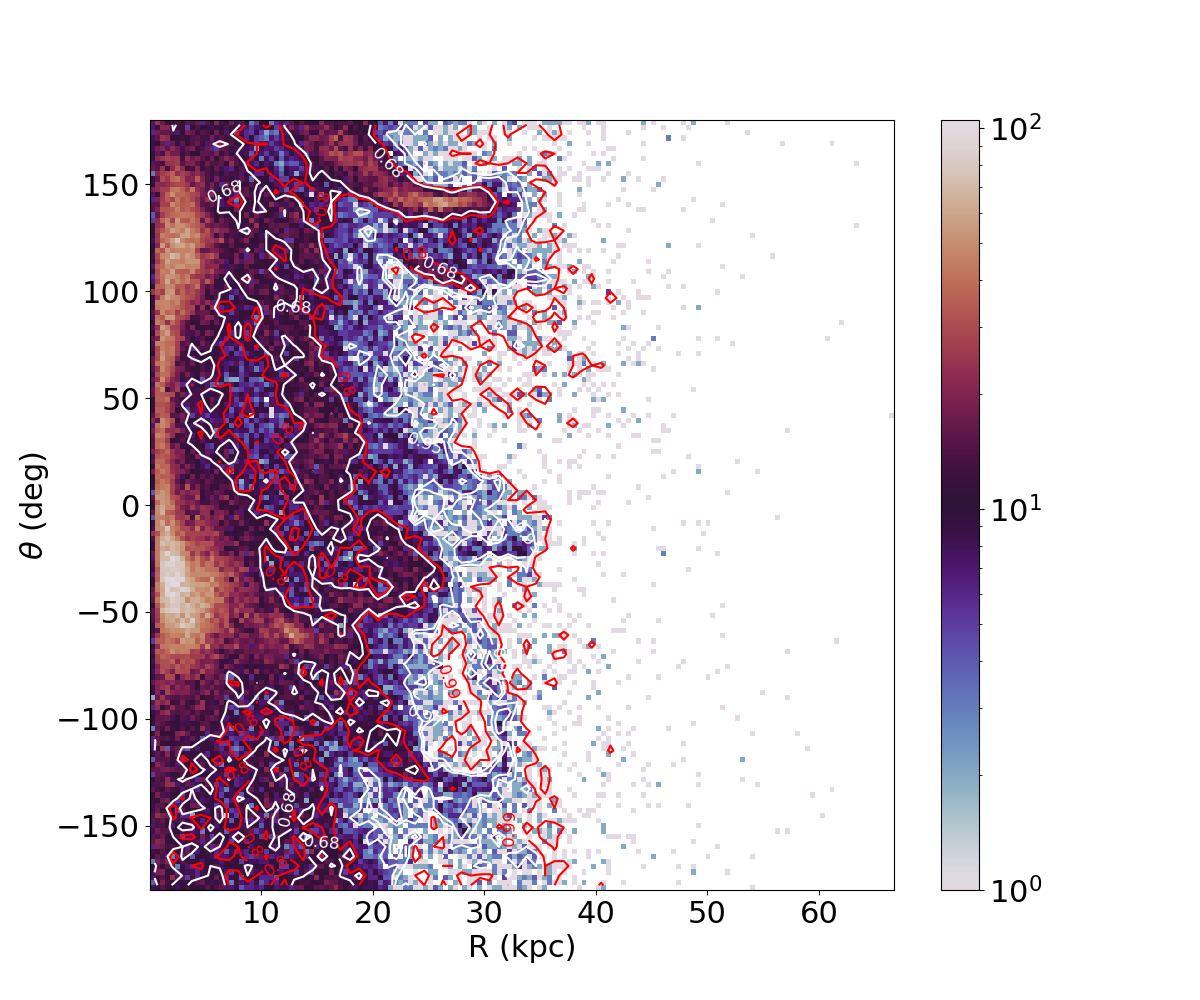
\includegraphics[width=0.75\linewidth]{Lab7_SpiralPhase.png}
    \caption{A phase diagram of a snapshot of M31 disk particle data. This is from the Lab 7 in-class assignment. Note the arm on the top of the paper; the outstretched material is considered to be prominent tidal debris.}
    \label{fig:enter-label}
\end{figure}

The core calculations in this project involve determining the positions and velocities of disk particles relative to their host galaxy's COM, as well as tracking the evolution of velocity dispersion in the tidal tails over time. To analyze the structure and kinematics of each galaxy, we first shift into a COM frame, computing both the position and velocity of the stellar disk relative to the COM using the methods developed in prior coursework. The total spatial separation of each particle from the galaxy center is calculated using the Euclidean distance formula:

\begin{equation}
    r = \sqrt{(x-x_{COM})^2 + (y-y_{COM})^2+ (z-z_{COM})^2}  
\end{equation}

where x,  y, and z are the particle’s coordinates and $x_{COM}$, $y_{COM}$ and $z_{COM}$ are the coordinates of the galaxy’s center of mass.

The total velocity relative to the galaxy's bulk motion is computed as:

\begin{equation}
    v = \sqrt{(v_x-v_x,_{COM})^2 + (v_y-v_y,_{COM})^2+ (v_z-v_z,_{COM})^2}  
\end{equation}
where $v_x$, $v_y$, and $v_z$ are the particle’s velocity components and $v_x,_{COM}$,  $v_y,_{COM}$, and $v_z,_{COM}$ are the velocity components of the galaxy’s COM. 

To identify tidal tails, phase diagrams will be made by plotting particle velocities against their galactocentric radii. Particles that significantly deviate from the expected rotation curve—particularly those with large velocities and/or located at large radii—are flagged as outliers and are interpreted as members of the tidal tails. For reference, the circular velocity of disk particles can be estimated using:
\begin{equation}
    V_c=\sqrt{\frac{GM(r)}{r}}
\end{equation}
where G is the universal gravitational constant, M(r) is the enclosed mass at radius r, and $V_c$ is the circular velocity. 

After selecting tidal tail particles based on their phase-space positions, they can be tracked across simulation snapshots using their unique particle IDs, and use this data to compute the velocity dispersion at each time step:

\begin{equation}
    \sigma^2 = \frac{1}{N} \Sigma(v_i-\bar{v})^2
\end{equation}
where $v_i$ are individual particle velocities, $\bar{v}$ is the mean velocity of the group, and N is the number of particles in the tail. This allows us to track the particles in the tidal structures across snapshots and better understand how the merger affects their internal kinematics.

To investigate how tidal tails evolve during the Milky Way–M31 merger and how their velocity dispersion changes over time, two types of plots will be generated. The first is a phase diagram (theta vs. radius) for disk particles in both galaxies. This type of plot was developed in Lab 7, and will help identify outlier particles that do not follow the main disk rotation curve. The second plot will graphing velocity dispersion for tidal tail particles of both galaxies over the time period which the snapshot represents, which will be during the first encounter. This figure will be generated using a function that tracks the same set of disk particle indices across successive snapshots and calculates their velocity dispersion at each time step. The plot will display velocity dispersion versus time. This will allow for testing of the hypothesis that tidal tails gain internal velocity spread as a result of repeated gravitational interactions. Together, these two plots will answer the core research question by showing both the \textit{structure} of the tidal tails (via phase space) and the \textit{dynamical evolution} of their kinematics (via dispersion growth).

The hypothesis for this project is that tidal tails gain internal velocity spread after the first encounter as a result of repeated gravitational interactions. This prediction is motivated by the expectation that repeated gravitational encounters and tidal stripping events will dynamically heat the outer regions of each galaxy's disk. As stars are pulled into extended tails, they become more susceptible to gravitational forces that are not only from the interaction with the companion galaxy but also from the evolving potential of the system as a whole. Unlike the inner disk, where stars follow relatively ordered, circular orbits, stars in the tails are no longer bound in a coherent structure and are more likely to exhibit random motions. This should manifest itself as a rise in velocity dispersion. Observing an increase in dispersion over time would allow for a better understanding on formation and evolution of tidal tails throughout a major merger. 

\section{Results}

This heatmap visualizes the distribution of disk stars in the Milky Way based on their radial distance (R, in kpc) and angular position ($\theta$, in degrees) at simulation snapshot 350. The color scale represents the number density of stars on a logarithmic scale, with darker shades indicating higher densities. Most stars are concentrated at radii less than 30 kpc, with a fairly symmetric spread in $\theta$. The low-density regions at large radii beyond \~50 kpc represent potential tidal features, including stars that have been ejected or disrupted during the galactic interaction. The main takeaway is that while the Milky Way disk remains mostly intact at this stage, there is visual evidence of low-density stellar material extending to large radii. This is consistent with the early formation of tidal tails.

This figure shows the time evolution of the velocity dispersion of tidal tail stars for both the Milky Way (red line) and M31 (blue line) from shortly before to after their first encounter, over a time span of roughly 3.5 to 5 Gyr. The y-axis shows the velocity dispersion in km/s, and the x-axis shows time in gigayears (Gyr). The dispersion values were computed based on stars identified as part of the tidal tails via phase space analysis. The plot highlights a pronounced peak in velocity dispersion for M31 near 4.15 Gyr, suggesting a strong dynamical response to the first passage. The Milky Way shows a more modest rise but a generally elevated dispersion through this period. The main takeaway is that the tidal tail particles from M31 experience a sharper increase in velocity dispersion during the first encounter, indicating a more violent disruption compared to the Milky Way disk.


\begin{figure}
    \centering
    \includegraphics[width=1\linewidth]{PhaseDiagram.png}
    \caption{Distribution of disk stars in the Milky Way based on their radial distance (R, in kpc) and angular position ($\theta$, in degrees) at simulation snapshot 350. The color scale represents the number density of stars on a logarithmic scale, with darker shades indicating higher densities. Note that while the Milky Way disk remains mostly intact at this stage, there is visual evidence of low-density stellar material extending to large radii—consistent with the formation of tidal tails }
    \label{fig:enter-label}
\end{figure}

\begin{figure}
    \centering
    \includegraphics[width=1\linewidth]{VelocityDispersion.png}
    \caption{Time evolution of the velocity dispersion of tidal tail stars for both the Milky Way (red line) and M31 (blue line) from shortly before to after their first encounter. The y-axis shows the velocity dispersion in km/s, and the x-axis shows time in gigayears (Gyr). M31's tidal tail particles experience a sharper increase in velocity dispersion during the first encounter, indicating a more violent disruption compared to the Milky Way disk.}
    \label{fig:enter-label}
\end{figure}

4. Each figure must have a detailed caption where everything plotted is explained, including axis labels and line types/colors. Include in the caption a punchline for each figure that explains what the reader should take away.



\section{Discussion}

1. Paragraph 1: Summarize one result from the previous section. Does this result agree or disagree with your hypothesis?

The results from the velocity dispersion plot show that after the first encounter between the Milky Way and M31, the tidal tails of both galaxies experience a noticeable increase in internal velocity dispersion. In particular, M31 exhibits a sharp rise in velocity dispersion around 4.15 Gyr, peaking significantly before a slight decline, while the Milky Way shows a more moderate but consistent elevation in dispersion during the same time frame. This trend supports the original hypothesis: repeated gravitational interactions and tidal forces during and after the first encounter dynamically heat the outer stellar populations, leading to a loss of ordered motion and an increase in random stellar velocities. The observed rise in dispersion is consistent with the expectation that stars pulled into tidal tails become increasingly kinematically disordered over time as the system evolves, confirming the idea that tidal tails are dynamically heated structures formed through repeated gravitational disturbances during a major merger.

2. Paragraph 2: How does the result from Paragraph 1 relate to existing work in the literature? E.g. the papers you cited in the introduction. What is the importance/meaning of this result for our understanding of galaxy evolution?

The observed increase in velocity dispersion of tidal tail stars following the first encounter is consistent with prior theoretical and simulation-based studies on galactic interactions. As described by Mihos (2004), tidal forces during close passages of galaxies inject energy into the disk, stretching material into tails and bridges. Our result empirically supports this by showing that such stretching is accompanied by dynamical heating, as measured by a rise in velocity dispersion. Furthermore, the results resonate with the foundational work of Toomre \& Toomre (1972), which established that the outer disk is most susceptible to tidal deformation during prograde encounters—precisely where dynamically hot tidal features are expected to form. Importantly, our findings also reinforce the critique raised by Privon et al. (2013), where test-particle simulations failed to capture realistic kinematics due to the omission of velocity dispersion. Our use of particle-tracked velocity dispersion directly illustrates the physical process that Privon et al. argued must be included for accurate modeling. This result deepens our understanding of galaxy evolution by emphasizing that tidal tails are not just morphological features, but dynamically complex structures whose internal kinematics evolve significantly as a consequence of repeated gravitational interactions. Recognizing this helps constrain models of stellar redistribution and star formation in merger remnants, contributing to a more complete picture of how large-scale structure forms in the universe.

3. Paragraph 3: What are the uncertainties in your analysis?

There are several sources of uncertainty in this analysis. One uncertainty arises from the identification of tidal tails by visual inspection of 2D histograms and phase diagrams. Since this step is subjective, it introduces the possibility of inconsistent or biased particle selection across snapshots. Additionally, identifying outliers in phase space is dependent on the definition that is set in place of what constitutes a significant deviation from the rotation curve. Thresholds may vary across snapshots due to the evolving structure of the disks. Temporal resolution of the simulation is another factor; if the time between snapshots is too large, important dynamical events that contribute to changes in velocity dispersion may be missed or under-sampled. Since the data was collected and graphed over intervals of 10 snapshots, the dispersion values themselves may be sensitive to contamination from disk particles that were not fully stripped, especially if the number of particles in the tidal tails is small. Lastly, without correcting for the COM motion or projection effects, some velocity measurements may include contributions from bulk motions rather than internal dispersion, which could artificially inflate the measured values. These uncertainties highlight the importance of refining selection criteria and possibly implementing automated or statistical methods to improve robustness.


\bibliographystyle{mnras}
\bibliography{example}

% Don't change these lines
\bsp	% typesetting comment
\label{lastpage}
\end{document}

% End of mnras_template.tex
